\chapter{Scripts and Images}
\section{CLI Flags}
\begin{figure}[h!]
\centering
\begin{BVerbatim}
PDDL Path Solver

options:
  -h, --help            show this help message and exit
  -d {blockly_maze,directional_maze,non_directional_maze,snake}, 
  --domain {blockly_maze,directional_maze,non_directional_maze,snake}
  -r DISPLAY_PROBLEMS, --display_problems DISPLAY_PROBLEMS
  -t {each,all}, --solution_type {each,all}
  -a, --auto
  -p PROBLEM_COUNT, --problem_count PROBLEM_COUNT
  -l PROGRAM_LINES, --program_lines PROGRAM_LINES
  -s TILE_SIZE, --tile_size TILE_SIZE
  -i IMAGE_DIRECTORY, --image_directory IMAGE_DIRECTORY
  -j PLAN_DIRECTORY, --plan_directory PLAN_DIRECTORY
  -k PROBLEM_DIRECTORY, --problem_directory PROBLEM_DIRECTORY
  -c APPLE_COUNT, --apple_count APPLE_COUNT
\end{BVerbatim}
\caption{Help text describing the usage of the program}
\end{figure}

\hfill
\section{Unified Planning Examples}
\subsection{Directional Maze Problem}
\newpage

\begin{figure}[h!]
\centering
\begin{BVerbatim}
problem name = reduced_maze0

types = [position]

fluents = [
  bool path[a=position, b=position]
  bool at[x=position]
]

actions = [
  action move(position x, position xn) {
    preconditions = [
      (at(x) and path(x, xn))
    ]
    effects = [
      at(xn) := true
      at(x) := false
    ]
  }
]

objects = [
  position: [start, goal, u0, ..., l14]
]

initial fluents default = [
  bool path[a=position, b=position] := false
  bool at[x=position] := false
]

initial values = [
  at(start) := true
  path(start, u0) := true
  ...
  path(r6, goal) := true
]

goals = [
  at(goal)
]
\end{BVerbatim}
\caption{Example Unified Planning instance}
\end{figure}

\newpage \hfill
\section{Images Used in Experiments}
\subsection{Problems with No Turns}

\begin{figure}[h!]
\centering

\includegraphics[width=0.7\textwidth]{experiment_images/p1.png}
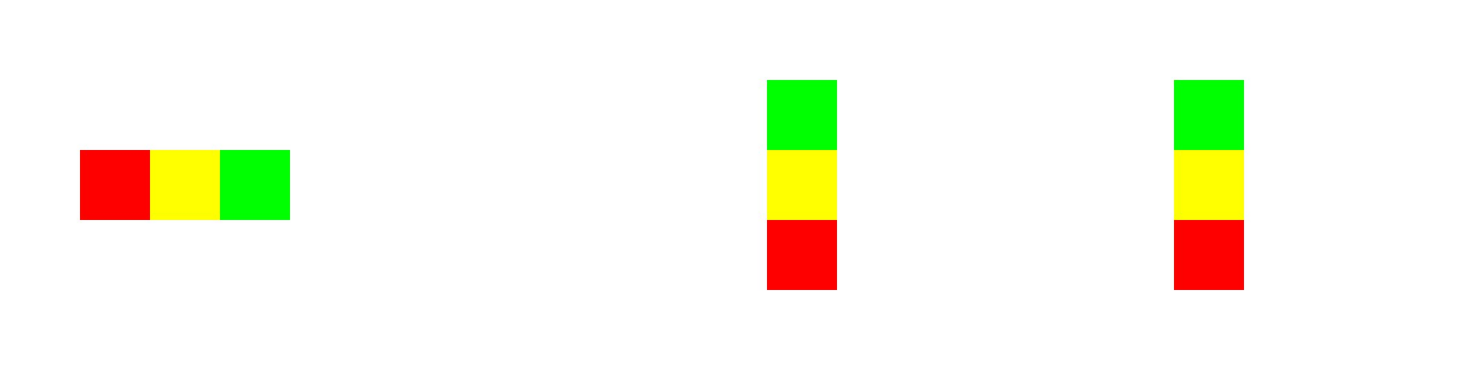
\includegraphics[width=0.7\textwidth]{experiment_images/p2.png}
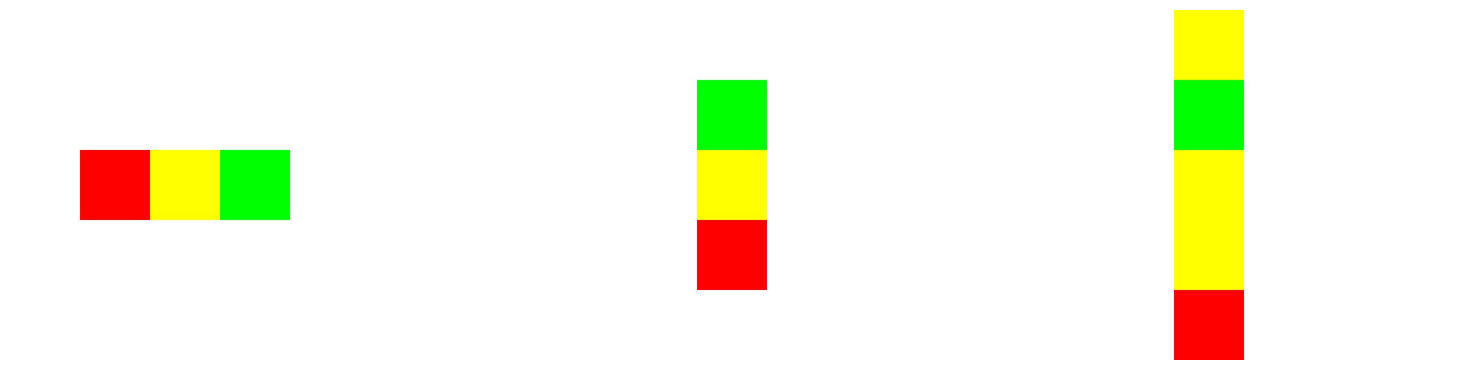
\includegraphics[width=0.7\textwidth]{experiment_images/p3.png}

\includegraphics[width=0.7\textwidth]{experiment_images/p4.png}
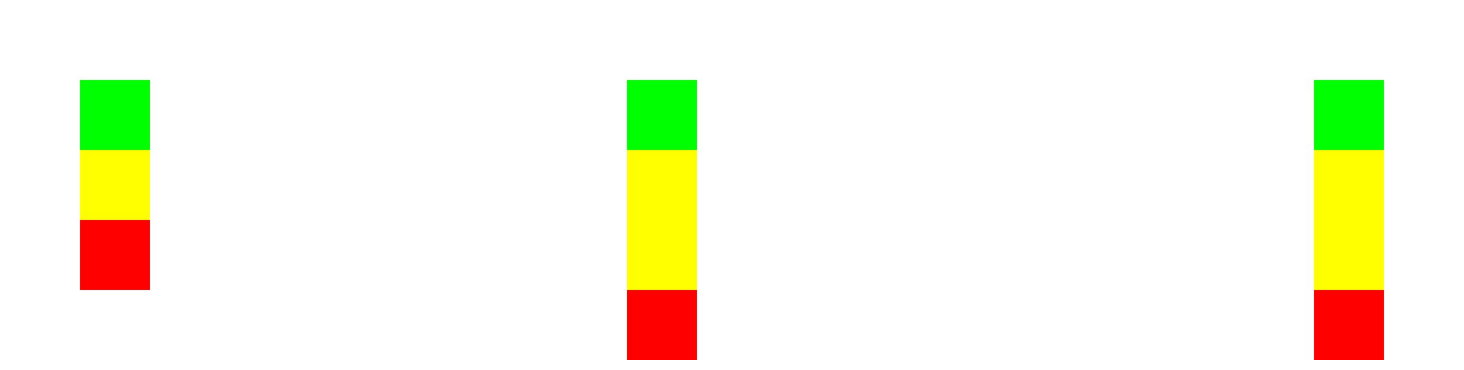
\includegraphics[width=0.7\textwidth]{experiment_images/p5.png}
\caption{Experiment images for "Problems with No Turns"}
\end{figure}

\newpage \hfill
\subsection{Identical Problems}

\begin{figure}[h!]
\centering

\includegraphics[width=0.7\textwidth]{experiment_images/i1.png}

\includegraphics[width=0.7\textwidth]{experiment_images/i2.png}

\includegraphics[width=0.7\textwidth]{experiment_images/i3.png}

\includegraphics[width=0.7\textwidth]{experiment_images/i4.png}
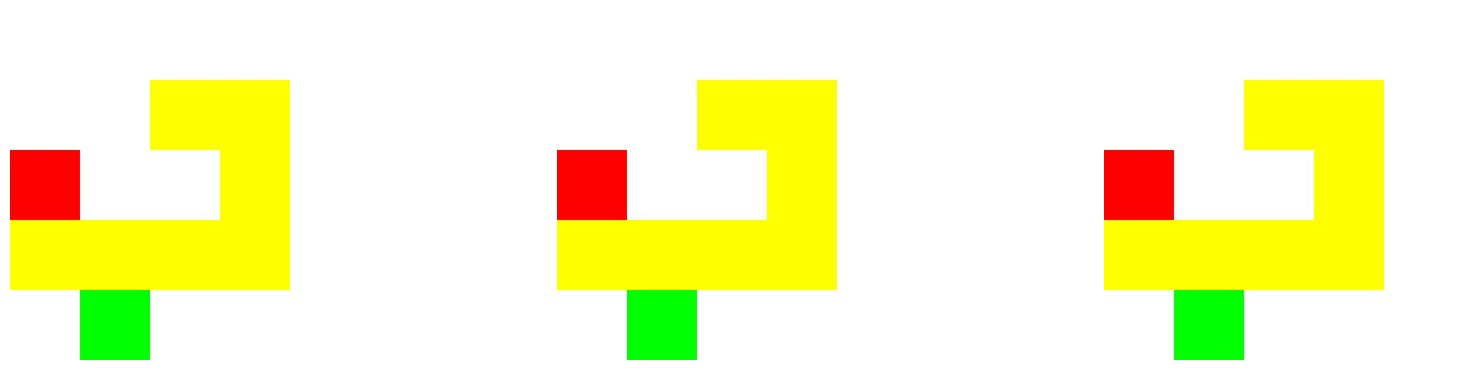
\includegraphics[width=0.7\textwidth]{experiment_images/i5.png}
\caption{Experiment images for "Identical Problems"}
\end{figure}